%!TEX root = Uno-Dokumentation.tex

\chapter{UNO}
\label{ch:uno}
Dieses Kapitel gibt einen Überblick über das Gesellschaftsspiel \textit{UNO}, welches in dieser Arbeit programmiert wird. Es wird ausschließlich auf die Punkte eingegangen, die benötigt werden um die Funktionen in der programmierten Software zu verstehen. \textit{UNO} ist ein Kartenspiel, geeignet für 2 - 10 Spieler ab einem Alter von 7 Jahren. Ziel des Spiels ist es, als erste Person alle Handkarten abgelegt zu haben.
\section{Karten}
\label{ch:karten}
Das standard-UNO-Kartendeck besteht aus 108 Karten, wie in Abbildung \ref{fig:uno_cards} zu sehen ist. Für die weitere Betrachtung werden die Karten in zwei Kategorien (Einfache Karten und Spezialkarten) eingeteilt. Zu den einfachen Karten gehören die nummerierten, die restlichen zu den Spezialkarten. 
\begin{figure}[h]
\begin{center}
	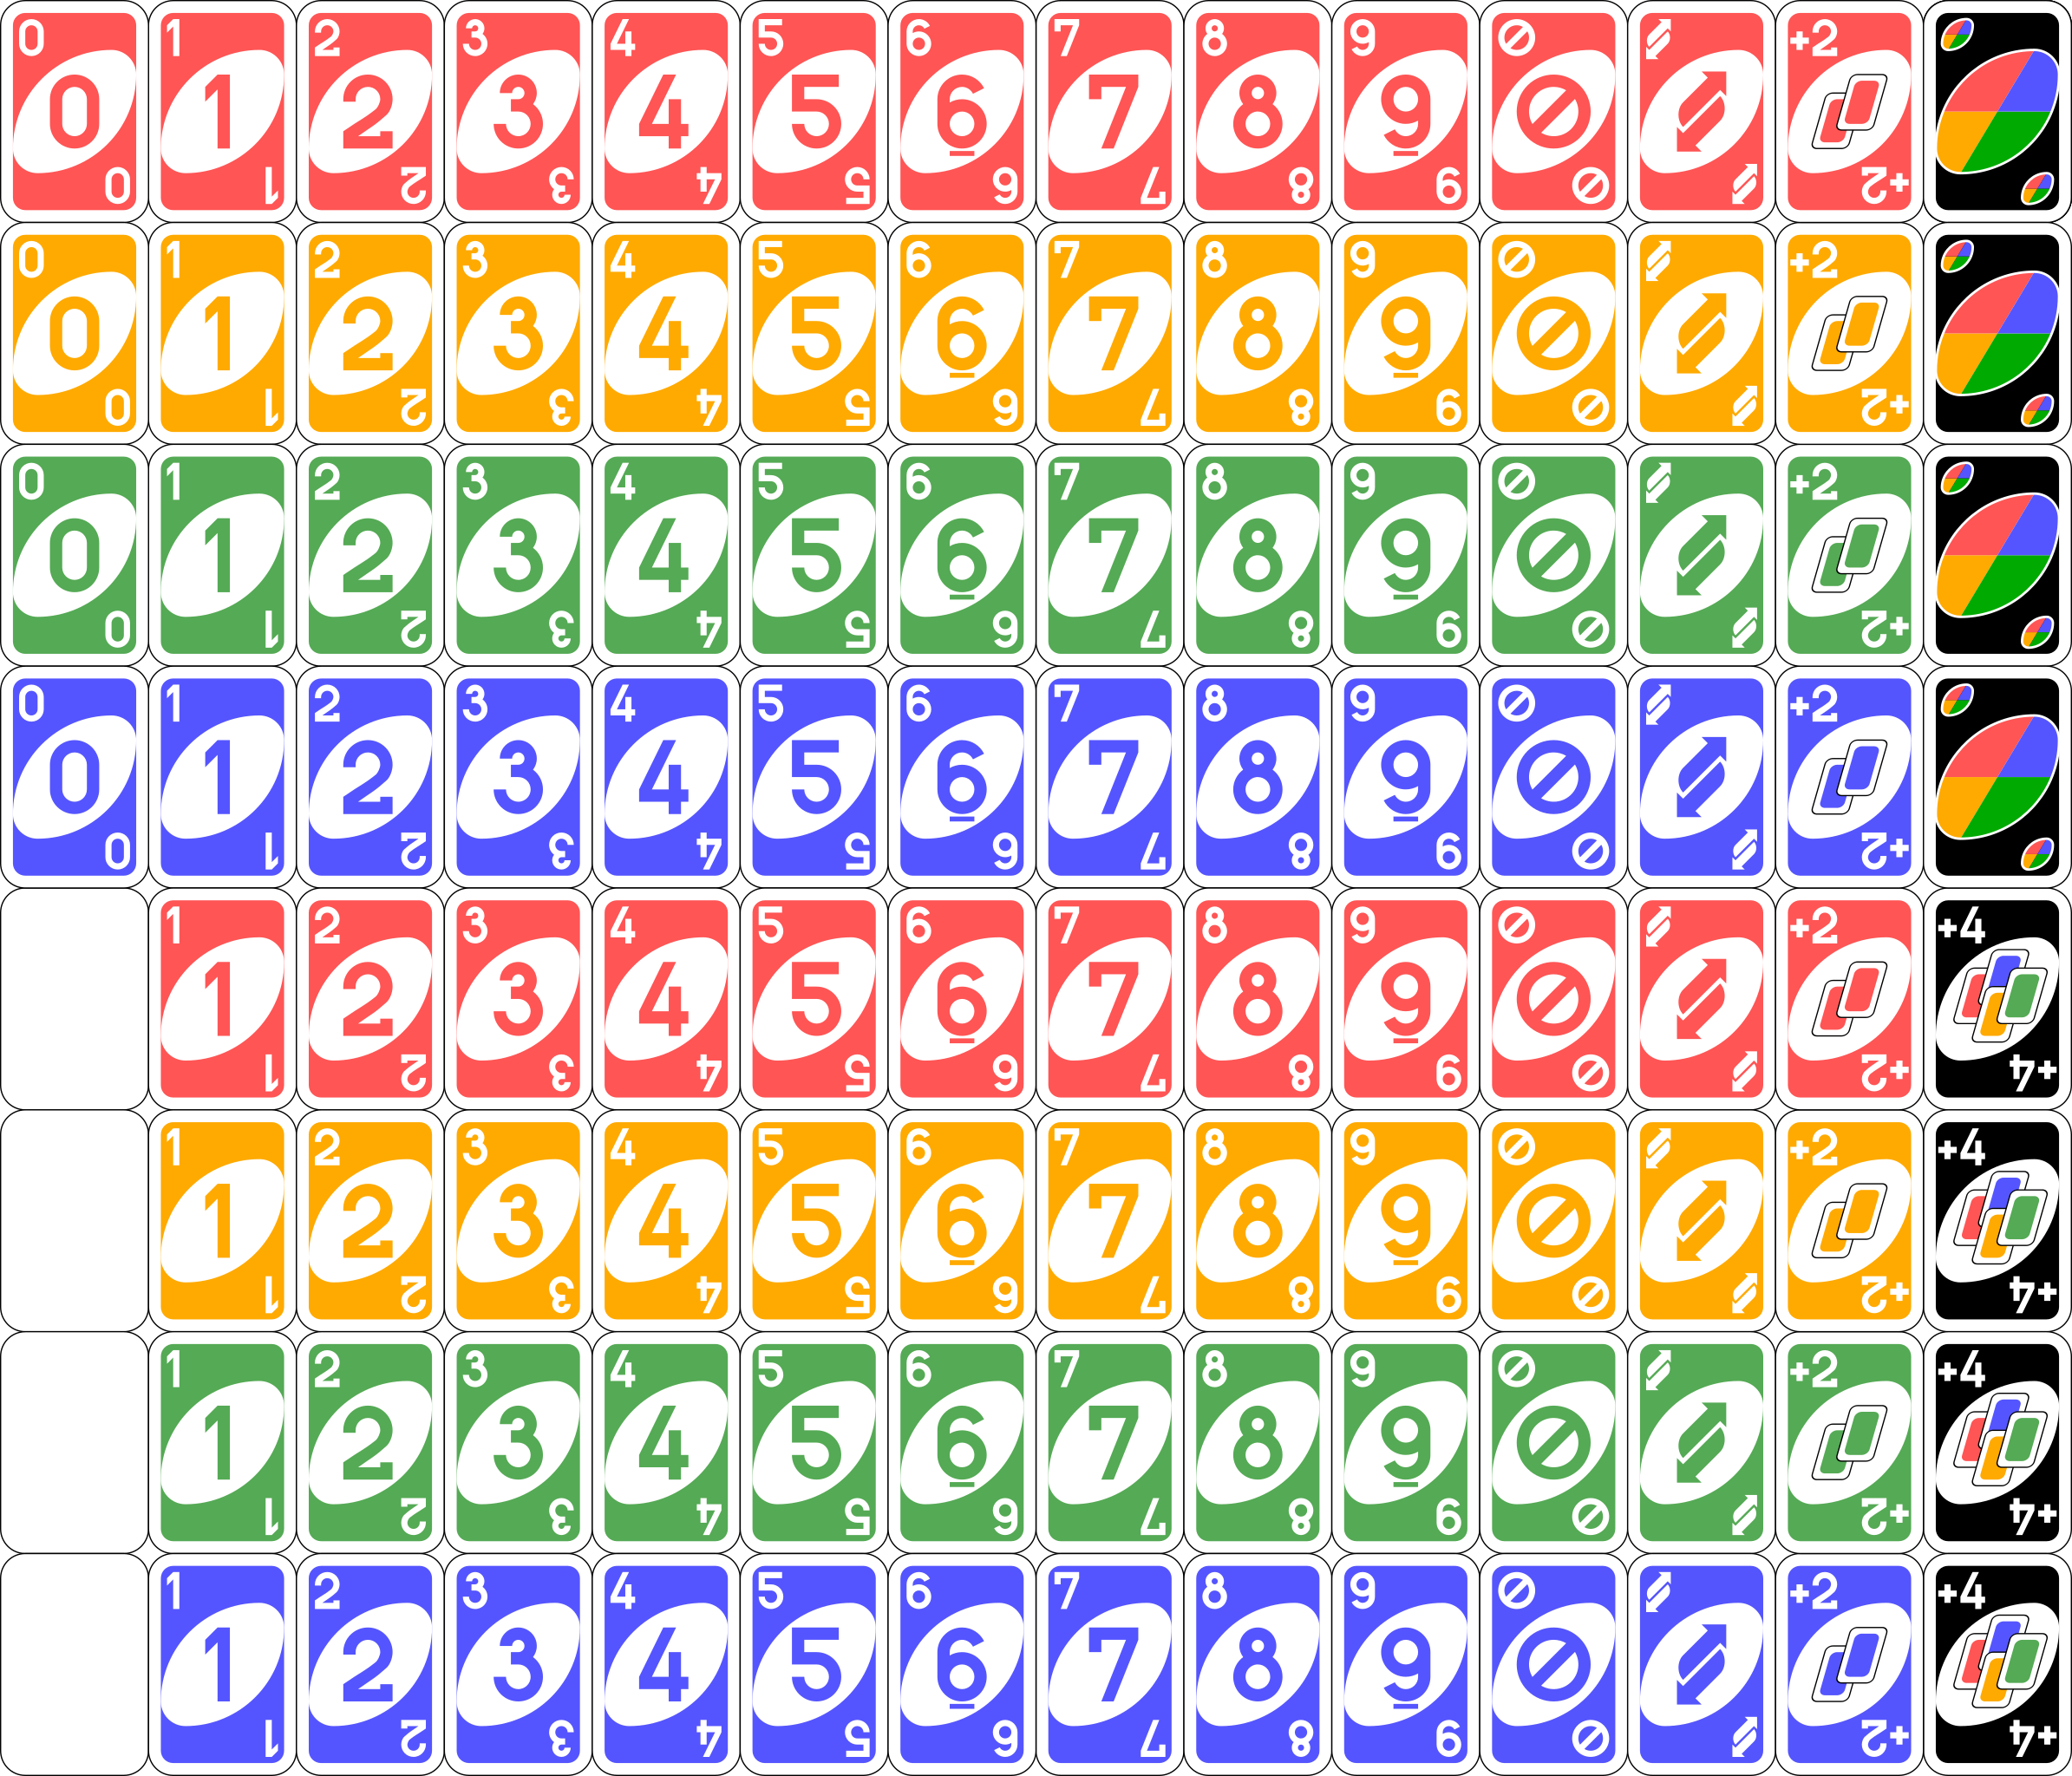
\includegraphics[width=.5\linewidth]{bilder/UNO_cards_deck.png}
	\caption{UNO Karten \\Quelle: https://shopping.mattel.com/de-de/products/uno-kartenspiel-w2087-de-de}
	\label{fig:uno_cards}
	%Quelle:  https://upload.wikimedia.org/wikipedia/commons/thumb/9/95/UNO_cards_deck.svg/2389px-UNO_cards_deck.svg.png
\end{center}
\end{figure}
Die einfachen Karten existieren in vier verschiedenen Farben. Jede Farb-Zahl-Kombination existiert zweimal, wobei die Karten mit einer null nur einmal existieren. Im Rahmen dieser Arbeit sind vorrangig nur die einfachen Karten von Bedeutung. Spezialkarten verändern das Spielgeschehen, indem zum Beispiel der nächste Spieler für eine Runde aussetzen muss, oder zwei Karten ziehen muss. \\
Zu Beginn des Spiels erhält jeder Spieler 7 Karten. In der Tischmitte wird eine Karte aufgedeckt platziert, auf dem die Spieler nach der Reihe Karten ablegen, oder ziehen können. Im folgenden wird auf die Spielregeln eingegangen.
\section{Spielregeln}
Ziel einer Runde ist es, als erster Spieler alle Handkarten auf den in der Tischmitte platzierten Kartenstapel abzulegen. Daraufhin werden die Wertungen der Karten der Gegenspieler addiert und dem Gewinner der Runde als Punkte gutgeschrieben. Der erste Spieler, der 500 Punkte erreicht, gewinnt das Spiel. Die Spieler sind nacheinander im Uhrzeigersinn an der Reihe. Eine Karte kann abgelegt werden, wenn entweder die Zahl oder die Farbe der abzulegenden Karte mit der Zahl oder Farbe der in der Tischmitte liegenden Karte übereinstimmt. Hat der Spieler keine passende Karte auf der Hand, so muss er eine neue Karte vom Stapel ziehen. Der Zug ist damit beendet. Hat ein Spieler nur noch eine Karte auf der Hand, so muss er dies mit dem Wort \textit{UNO} den anderen Spielern mitteilen. Wird die letzte Karte ohne diese Aussage abgelegt, so muss die Karte wieder aufgenommen und eine weitere Strafkarte vom Stapel gezogen werden. Daraufhin ist der Zug beendet \cite{UnoRules}. Die Regeln bezüglich der Spezialkarten sind im Rahmen dieser Arbeit nicht von Bedeutung.